\section{Geometric realization and local diagnostics}
\label{sec:geometric-realization}

% Audited foundation; deterministic figure integrated 2026-10-30.

\subsection{Pairwise separators and realized faces}
\label{subsec:faces}

For a finite nonperiodic configuration, the \emph{power cell} $C_i(w)$ of site $i$ consists of all points at which its power distance is minimal among the sites \cite{Aurenhammer1987}. For two distinct sites $i$ and $j$, we distinguish their \emph{pairwise bisector} $H_{ij}(w)$, where their power distances are equal, from their \emph{common cell intersection} $F_{ij}(w)$, where both sites attain the minimum power distance. Explicitly,
\begin{align}
C_i(w)&=\{x\in\mathbb R^d:\pi_i(x)\le\pi_k(x)
\text{ for all }k\}, \label{eq:power-cell}\\[2pt]
H_{ij}(w)&=\{x\in\mathbb R^d:\pi_i(x)=\pi_j(x)\}, \label{eq:pair-bisector}\\[2pt]
F_{ij}(w)&=C_i(w)\cap C_j(w)\notag\\
&=\{x\in H_{ij}(w):
\pi_i(x)\le\pi_k(x)
\text{ for all }k\ne i,j\}. \label{eq:common-cell-intersection}
\end{align}

While the position of $H_{ij}$ depends only on the weight difference $w_i-w_j$, the existence and extent of $F_{ij}$ depend on the competing sites and their weights. In particular, $F_{ij}$ may be empty even when the pairwise separator is fitted exactly. Moreover, a nonempty intersection need not form a full $(d-1)$-dimensional face: the two cells may meet only in a lower-dimensional set.

Recall that Section~2 describes the position of a pairwise separator by its coordinate along the line through the two sites. For fitted weights, this identifies a particular point on the pairwise bisector,
\begin{equation}
q_{ij}(w)=p_i+t_{ij}(w)(p_j-p_i)\in H_{ij}(w).
\label{eq:connector-point}
\end{equation}
This gives a second geometric question beyond the existence of a shared face: does this particular point belong to the common cell intersection $F_{ij}$? The condition $q_{ij}\in F_{ij}$ is stronger than $F_{ij}\ne\varnothing$, since a shared face may lie elsewhere on the bisector. The following example illustrates both distinctions.

Consider four sites in the plane,
\begin{equation}
p_1=(0,0),\quad p_2=(2,0),\quad
p_3=(1,1),\quad p_4=(1,-1),
\label{eq:four-sites}
\end{equation}
with $w_1=w_2=0$. The pairwise bisector of sites 1 and 2 is always $H_{12}=\{(1,y):y\in\mathbb R\}$, and its intersection with the line through the two sites is $q_{12}=(1,0)$, regardless of the weights assigned to sites 3 and 4. The conditions imposed by these competing sites give
\begin{equation}
F_{12}=\left\{(1,y):
\frac{w_4}{2}\le y\le-\frac{w_3}{2}\right\}.
\label{eq:four-site-face}
\end{equation}

Figure~\ref{fig:three-face-cases} shows how changing only the competing weights makes the shared face disappear, moves it away from the connector, or places the connector point inside it.

\begin{figure}[!tb]
\centering
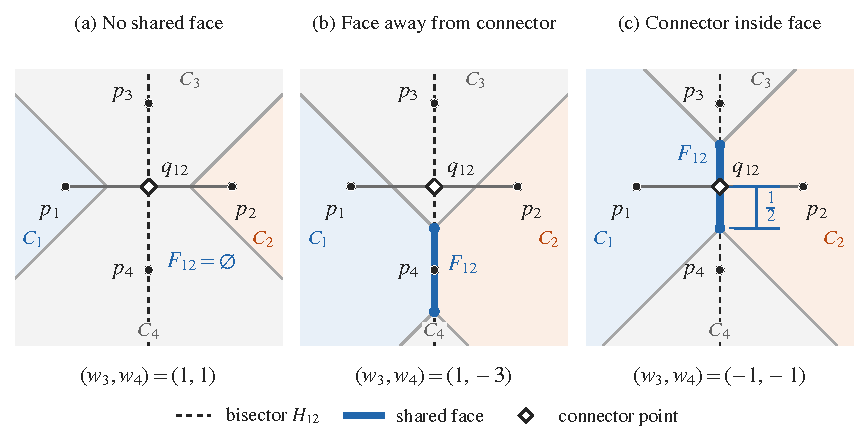
\includegraphics[width=\linewidth]{figures/figure_04_realization.pdf}
\caption{Three outcomes for the fixed sites in Eq.~\eqref{eq:four-sites}, with $w_1=w_2=0$. The dashed bisector $H_{12}$ and diamond $q_{12}$ stay fixed. Shading distinguishes the power cells; the blue segment shows $F_{12}$ when it is nonempty. (a) $F_{12}=\varnothing$. (b) $F_{12}=\{1\}\times[-3/2,-1/2]$, away from $q_{12}$. (c) $F_{12}=\{1\}\times[-1/2,1/2]$, with $q_{12}$ strictly inside; the bracket measures the distance $1/2$ to an endpoint. Site markers need not lie in their own cells: in (b), $p_4\in F_{12}$ but $p_4\notin C_4$. All panels use the same scale and drawing window; the cells are defined in the full plane.}
\label{fig:three-face-cases}
\end{figure}

Since $F_{ij}$ lies in the $(d-1)$-dimensional hyperplane $H_{ij}$, it contains a full $(d-1)$-dimensional portion precisely when
\begin{equation}
\boxed{\operatorname{int}_{H_{ij}}F_{ij}\ne\varnothing,}
\label{eq:full-dimensional-face}
\end{equation}
where $\operatorname{int}_{H_{ij}}$ denotes interior within the entire bisector hyperplane. Equivalently, $F_{ij}$ must contain a nonempty open ball measured within $H_{ij}$. When both power cells are themselves full-dimensional, such an intersection is a shared facet of the two cells.

The distinction is visible in the four-site example. With $(w_3,w_4)=(1,-1)$, the bounds defining $F_{12}$ meet at $y=-1/2$, leaving only the point $(1,-1/2)$. The cells intersect, but they do not share an edge.

Further degeneracies are discussed in~\ref{app:geometry-degeneracy}. We next test connector membership using power-distance comparisons.

\subsection{Connector visibility}
\label{subsec:connector-visibility}

The fitted separator coordinate fixes $q_{ij}$, so testing $q_{ij}\in F_{ij}$ checks geometric support at that location without searching for another witness on the bisector.

To perform this test, we compare the power distances of the pair with those of the competing sites at $q_{ij}$. For each $k\notin\{i,j\}$, define the \emph{competitor gap}
\begin{equation}
g_{ijk}(w)=\pi_k(q_{ij}(w))-\pi_i(q_{ij}(w)).
\label{eq:competitor-gap}
\end{equation}
Since $\pi_i(q_{ij})=\pi_j(q_{ij})$, the point belongs to both power cells exactly when no competitor has a smaller power distance. Thus,
\begin{equation}
\boxed{q_{ij}(w)\in F_{ij}(w)
\quad\Longleftrightarrow\quad
g_{ijk}(w)\ge0
\quad\text{for all }k\notin\{i,j\}.}
\label{eq:weak-connector-visibility}
\end{equation}

We refer to this as \emph{weak connector visibility}. Strict positivity of every competitor gap provides a stronger certificate: for a finite configuration, the inequalities remain satisfied in a neighborhood of $q_{ij}$ within the bisector. Consequently,
\begin{equation}
g_{ijk}(w)>0\quad\text{for all }k\notin\{i,j\}
\quad\Longrightarrow\quad
q_{ij}(w)\in\operatorname{int}_{H_{ij}}F_{ij}(w).
\label{eq:strict-connector-visibility}
\end{equation}
Strict competitor inequalities also persist in a small ambient neighborhood of $q_{ij}$. On opposite sides of the bisector near that point, sites $i$ and $j$, respectively, are the unique power minimizers. Thus strict visibility certifies a genuine local facet between two full-dimensional cells.

When all site weights are equal, $q_{ij}$ is the midpoint, and strict positivity of the gaps means that every other site lies outside the closed ball with diameter $p_ip_j$. This is the strict form of the classical \emph{Gabriel} edge condition. Its weighted counterpart uses the full affine connector line, so the witness may lie outside the site segment \cite[Sec.~2]{Alexa2020}. The all-strict test above is therefore a weighted Gabriel edge certificate. We use \emph{weak connector visibility} separately for the non-strict condition $q_{ij}\in F_{ij}$, which permits boundary contacts and persistent ties and does not by itself certify a genuine facet; see~\ref{app:geometry-degeneracy}.

The competitor gaps can be expressed directly in terms of the fitted weights. Writing $\delta_{ij}=p_j-p_i$ and $q_{ij}=p_i+t_{ij}\delta_{ij}$, expansion of the squared distances gives
\begin{equation}
g_{ijk}(w)=
\|p_k-p_i\|^2
-2t_{ij}(w)\,\delta_{ij}\cdot(p_k-p_i)
+w_i-w_k.
\label{eq:gap-affine-formula}
\end{equation}
Since $t_{ij}(w)$ is affine in $w_i-w_j$, each competitor gap is an affine function of the site weights for fixed site positions. It is also invariant under adding a common constant to all weights.

For a pair $i,j$, we summarize the competitor inequalities by the \emph{minimum signed gap}
\begin{equation}
\boxed{\sigma_{ij}(w)=\min_{k\notin\{i,j\}}g_{ijk}(w).}
\label{eq:minimum-signed-gap}
\end{equation}
When there are no competing sites, we set $\sigma_{ij}=+\infty$. Otherwise, $\sigma_{ij}$ is a continuous, piecewise-affine function of the weights. The weak connector-visibility condition is equivalent to $\sigma_{ij}\ge0$, while $\sigma_{ij}>0$ guarantees strict visibility and a full-dimensional shared face near $q_{ij}$. A negative value only establishes that the selected connector point is not on the shared face; it does not exclude a face elsewhere on the bisector.

In Fig.~\ref{fig:three-face-cases}(a--c), the values of $\sigma_{12}$ are respectively $-1$, $-1$, and $+1$. The same negative score occurs both when the face is absent and when it lies away from the connector.

\subsection{Connector-centered clearance}
\label{subsec:connector-clearance}

A strictly positive minimum signed gap $\sigma_{ij}$ places the connector point in the interior of $F_{ij}$ within the bisector. The gap has units of squared length, however, and does not directly describe the geometric extent of this interior neighborhood.

When $q_{ij}\in F_{ij}$, we define the \emph{connector-centered clearance} $c_{ij}$ as the supremum of radii $r\ge0$ for which the in-bisector Euclidean ball
\begin{equation}
B_{H_{ij}}(q_{ij},r)
=\{q_{ij}+u:
u\cdot\delta_{ij}=0,\ \|u\|\le r\}
\label{eq:bisector-ball}
\end{equation}
is contained in $F_{ij}$. This is a ball of dimension $d-1$, with the Euclidean metric inherited from $\mathbb R^d$, and its center is fixed at $q_{ij}$.

Let $e_{ijk}$ be the component of $p_k-p_i$ perpendicular to the site connector:
\begin{equation}
e_{ijk}
=(p_k-p_i)
-\frac{(p_k-p_i)\cdot\delta_{ij}}
{\|\delta_{ij}\|^2}\delta_{ij}.
\label{eq:projected-competitor}
\end{equation}
For any displacement $u$ within the bisector, the difference of power distances becomes
\begin{equation}
\pi_k(q_{ij}+u)-\pi_i(q_{ij}+u)
=g_{ijk}-2e_{ijk}\cdot u.
\label{eq:power-gap-displacement}
\end{equation}

The smallest value of this expression over $B_{H_{ij}}(q_{ij},r)$ is $g_{ijk}-2r\|e_{ijk}\|$. Thus, the entire ball is contained in the common cell intersection exactly when
\begin{equation}
2r\|e_{ijk}\|\le g_{ijk}
\qquad\text{for every competitor }k.
\label{eq:clearance-inequalities}
\end{equation}
It follows that, for $\sigma_{ij}>0$,
\begin{equation}
\boxed{
c_{ij}(w)=
\min_{\substack{k\notin\{i,j\}\\\|e_{ijk}\|>0}}
\frac{g_{ijk}(w)}{2\|e_{ijk}\|}.
}
\label{eq:connector-clearance}
\end{equation}
The minimum over an empty set is $+\infty$, corresponding to $F_{ij}=H_{ij}$. Under strict visibility, competitors with $e_{ijk}=0$ impose no restriction on motion within the bisector.

In Fig.~\ref{fig:three-face-cases}(c), both competitor gaps and both projected distances equal $1$. Hence $c_{12}=1/2$, the marked distance from $q_{12}$ to an endpoint of the shared edge.

% PRO-REVIEW: Is the exterior-distance discussion sufficiently motivated
% and economical, given the planned implementation-level usage?
The formula should not be extended to negative gaps by simply allowing a negative clearance. When $\sigma_{ij}<0$, the connector point lies outside $F_{ij}$, so no centered ball, not even one of radius zero, is contained in the common cell intersection. Moreover, a negative value of the expression above describes a violation of an individual competitor inequality, whereas the distance to the actual face depends on satisfying all inequalities simultaneously. The face may even be empty.

For a nonempty face, the appropriate exterior measure is instead the Euclidean distance from $q_{ij}$ to $F_{ij}$, measured within the bisector. In~\ref{app:geometry-exterior}, we derive its computation as a convex projection problem and illustrate why a negative extension of Eq.~\eqref{eq:connector-clearance} does not generally give this distance. The zero-gap clearance formula is treated in~\ref{app:geometry-exterior}; persistent ties are discussed in~\ref{app:geometry-degeneracy}. 

\subsection{Stability of geometric support}
\label{subsec:geometric-stability}

The diagnostics above refer to a particular set of fitted weights. Errors in separator observations can perturb these weights, so we ask when the resulting connector-visibility classification remains stable.

We first consider a fixed finite, nonperiodic site configuration. For a pair $i,j$ and competitor $k$, define the dimensionless coefficient
\begin{equation}
\theta_{ijk}
=\frac{(p_k-p_i)\cdot(p_j-p_i)}
{\|p_j-p_i\|^2}.
\label{eq:stability-theta}
\end{equation}
This is the coordinate of the orthogonal projection of $p_k$ onto the affine line through $p_i,p_j$. From the affine expression for the competitor gap in Section~4.2, a weight perturbation $\Delta w$ gives the exact identity
\begin{equation}
g_{ijk}(w+\Delta w)-g_{ijk}(w)
=(1-\theta_{ijk})\Delta w_i
+\theta_{ijk}\Delta w_j-\Delta w_k.
\label{eq:gap-weight-perturbation}
\end{equation}
Consequently, defining
\begin{equation}
K_{ij}=
\max_{k\notin\{i,j\}}
\left(
|1-\theta_{ijk}|+|\theta_{ijk}|+1
\right),
\label{eq:gap-lipschitz-constant}
\end{equation}
we obtain
\begin{equation}
\boxed{
|\sigma_{ij}(w+\Delta w)-\sigma_{ij}(w)|
\le K_{ij}\|\Delta w\|_\infty.
}
\label{eq:gap-lipschitz-bound}
\end{equation}
Here the competitor set is assumed nonempty. The bound follows because each competitor gap satisfies the corresponding estimate and taking the minimum cannot increase the largest absolute change.

In particular, if $\sigma_{ij}(w)>0$ and
\begin{equation}
K_{ij}\|\Delta w\|_\infty<\sigma_{ij}(w),
\label{eq:strict-stability-condition}
\end{equation}
then $\sigma_{ij}(w+\Delta w)>0$. Thus, the pair retains strict connector visibility, and its common face remains full-dimensional near the perturbed connector point.

The same argument preserves a negative sign when the perturbation bound is smaller than $|\sigma_{ij}(w)|$. This only certifies that the connector point remains outside the shared face; it does not establish that the face is absent. At zero margin, the bound provides no sign-preservation guarantee.

Because the competitor gaps are invariant under a common shift of all site weights, the perturbation bound may also be expressed using the smallest infinity norm after subtracting such a shift. The result concerns the connector-visibility status of the selected pair, not the topology of the entire power diagram.

The preceding bound concerns perturbations of the site weights. To relate it to errors in the observed separators, consider the unconstrained quadratic fit of Section~3 with a fixed observation graph and fixed positive fitting weights.

Let $z^\star$ be a reference vector of target differences, not necessarily compatible, and let $\widehat z=z^\star+\eta$ be a perturbed observation vector. Denote their least-squares solutions by $w^\star$ and $\widehat w$, respectively, using the same fixed linear convention for the undetermined component offsets. For this fixed fitting problem, the solution depends linearly on the targets. Writing this dependence as $w=Gz$, we obtain
\begin{equation}
\widehat w-w^\star=G\eta.
\label{eq:weight-response}
\end{equation}
Combining this identity with the geometric perturbation bound gives
\begin{equation}
\boxed{
|\sigma_{ij}(\widehat w)-\sigma_{ij}(w^\star)|
\le K_{ij}\|G\eta\|_\infty
\le K_{ij}\|G\|_{\infty\to\infty}\|\eta\|_\infty.
}
\label{eq:observation-to-visibility}
\end{equation}
If the right-hand side is smaller than $|\sigma_{ij}(w^\star)|$, the connector-visibility score keeps its sign.

The conclusion concerns the visibility classification of the \emph{reference least-squares fit}. It does not automatically establish agreement with an independently specified physical weight vector: any difference between that vector and the reference fit must also be accounted for. Moreover, when the observation graph is disconnected, the chosen component offsets affect the geometry, so the comparison requires a consistent convention. The reduced-Laplacian response and error bounds are given in~\ref{app:stability-estimator}; the additional bias when comparing with independent physical reference weights is treated in~\ref{app:stability-reference}.

\paragraph{Clipping and periodic images}
The preceding stability results concern a fixed finite set of sites in an unbounded nonperiodic domain. Clipping and periodicity require additional geometric qualifications.

For a diagram restricted to a convex box $\Omega$, the relevant common cell intersection is
\begin{equation}
F_{ij}^{\Omega}=F_{ij}\cap\Omega.
\label{eq:clipped-face}
\end{equation}
Strictly positive competitor gaps alone do not guarantee that the connector point belongs to this clipped intersection: the point must also lie inside $\Omega$. If $\sigma_{ij}>0$ and $q_{ij}\in\operatorname{int}\Omega$, then a neighborhood of $q_{ij}$ within the bisector belongs to $F_{ij}^{\Omega}$. The corresponding connector-centered clearance is
\begin{equation}
c_{ij}^{\Omega}
=\min\{c_{ij},b_{ij}^{\Omega}\},
\label{eq:clipped-clearance}
\end{equation}
where $b_{ij}^{\Omega}$ is the largest radius of an in-bisector ball centered at $q_{ij}$ and contained in $\Omega$. Intersections confined to the domain boundary require additional care, since an intersection of positive dimension within the bisector need not represent an interface between two full-dimensional cells inside the domain.

For periodic diagrams, the pairwise separator is associated with two selected site images, rather than merely their base-site indices. Every other image can act as a competitor, including other images of either selected base site. The power-gap and clearance constructions remain applicable to these image instances, but their evaluation requires the relevant competing images to be identified correctly. In particular, neither an arbitrary finite image cutoff nor the finite-competitor stability bound derived above is automatically valid for the complete periodic diagram.

See~\ref{app:geometry-clipping} for clipping and~\ref{app:geometry-periodic} for image-aware geometry. Further limitations on periodic perturbation bounds are recorded in~\ref{app:stability-periodic}.

These diagnostics characterize local geometric support of fitted separators. They complement, rather than replace, an explicit examination of the realized power diagram, which forms part of the computational workflow described next.
